%!TEX encoding = UTF-8 Unicode
\documentclass{reqenglecture}

\title{Introduction to Software Requirements Engineering}

\subtitle{Part 1: Domain Knowledge}

\author{Björn Regnell}

\date{\vspace{1em}\footnotesize Updated: \today~
\\ License: CC-BY-SA 
\\ \url{https://github.com/bjornregnell/reqeng-book} 
}

%\beamerdefaultoverlayspecification{<+->} %de-comment if you want pause after items

\begin{document}
\maketitle

\begin{frame}
\frametitle{Part 1: Domain Knowledge}
\framesubtitle{Outline}
\tableofcontents
\end{frame}


\LectureOnly{\section{Introduction}}

\begin{Slide}{What is Requirements Engineering (RE)?}

\begin{itemize}
\item RE is focused on the
\begin{itemize}
\item \textbf{features} of software-intensive systems 
\item \textbf{system context}, including users and connected systems
\item \textbf{development context}, including stakeholders' intentions 

\end{itemize}
\item The RE process involves 
\begin{itemize}
\item knowledge-building \hfill research
\item consensus-building \hfill agree
\item decision-making    \hfill choose
\item innovation         \hfill generate ideas
\item communication      \hfill be pedagogical

\end{itemize}
\end{itemize}
\end{Slide}

\begin{Slide}{What is a requirement?}

\begin{itemize}
\item Something \textbf{needed} or \textbf{wanted}.

\item A documented \textbf{representation} of\\something needed or wanted.
\item The word ''requirement'' have different meanings:\\
  must, wish, idea, specific design, rationale, ...

\item The most \textbf{general meaning}:\\
  \textit{any} kind of \textbf{information entity} used in RE

\item You don't always get what you want and you often want things that you don't need...

\end{itemize}
\end{Slide}

\begin{Slide}{Main Activities of RE}

{\vspace{1em}\resizebox{!}{3em}{\hspace{0.5em}{\bf ?}\hspace{0.5em}\WritingHand\hspace{0.5em}\Checkedbox\hspace{0.5em}\LeftScissors}\vspace{0.5em}}

\begin{itemize}
\item The 4 main activities of RE: 
\begin{itemize}
\item \textbf{Elicitation} \hfill learning
\item \textbf{Specification} \hfill representing
\item \textbf{Validation}  \hfill checking
\item \textbf{Selection}   \hfill deciding
\end{itemize}
\item These activities are
\begin{itemize}
\item \textbf{Interdependent} \hfill output of one is input to other activities
\item \textbf{Concurrent} \hfill one activity you often trigger another
\item \textbf{Continuous} \hfill in the product life-cycle as software evolves

\end{itemize}
\end{itemize}
\end{Slide}

\begin{Slide}{What is good RE?}

\begin{itemize}
\item Feasible and helpful foundation for software development
\item Cost-effective process with high artifact quality
\item Happy stakeholders
\item Good system 
\begin{itemize}
\item commercially successful
\item beneficial to its users
\item ethical, helpful to society
\end{itemize}
\item When are we ready? What is good enough?

\end{itemize}
\end{Slide}

\begin{Slide}{RE in the Development Process}

\begin{itemize}
\item RE interprets stakeholders intentions into validated req specs
\item RE provides input to, and learns from down-stream activities
\begin{itemize}
\item System Design
\begin{itemize}
\item Quality reqs determine architectural decisions
\end{itemize}
\item System Implementation
\begin{itemize}
\item Functional reqs (data and logic) are realized in code  
\end{itemize}
\item System Verification 
\begin{itemize}
\item The req spec define correct output in test cases
\end{itemize}
\item System Operation
\begin{itemize}
\item User feedback is input to requirements evolution
\end{itemize}
\end{itemize}
\item As requirements evolve you must manage impact of changes
\item Traceability: 
\begin{itemize}
\item Links among artifacts to support change management
\item Forwards: from requirements to down-stream activities
\item Backwards: from requirements to stakeholders

\end{itemize}
\end{itemize}
\end{Slide}

\begin{Slide}{Requirements as Solution Constraints}

\begin{itemize}
\item U: the \textbf{universe} of all possible software systems

\item S: the \textbf{solution space}, a subset of U including\\all systems that \textbf{fulfill the spec}

\item S contains both ''\textbf{good}'' and ''\textbf{bad}'' systems

\item The \textbf{general purpose} of RE:
\begin{itemize}
\item to \textbf{constrain the solution space} so that software development is likely to produce a \textbf{good enough} solution

\end{itemize}
\item The req spec should be a good enough definition of what we mean with a ''good enough solution''

\item RE is the \textbf{foundation for software quality}.



\end{itemize}
\end{Slide}

\begin{Slide}{Common Acronyms}

\begin{itemize}
\item RE   \hfill requirements engineering
\item SE   \hfill software engineering
\item req  \hfill requirement 
\item spec \hfill specification
\item SRS  \hfill software (or system) requirements specification
\item sys  \hfill system
\item SW   \hfill software
\item dev  \hfill development
\item ops  \hfill operations
\item FR   \hfill quality requirements
\item QR   \hfill functional requirements



\end{itemize}
\LectureOnly{\section{Purpose}}
\end{Slide}


\begin{Slide}{What is a Requirements Specification?}

\begin{itemize}
\item A collection of requirements models with supporting information to help interpretation

\item Expressed in a combination of suitable styles:
\begin{itemize}
\item natural language
\item formal language (controlled syntax and semantics)
\item diagrams
\item tables
\item pictures
\item videos
\item prototypes
\item ...

\end{itemize}
\item Similar to a shopping list:
\begin{itemize}
\item You don't always get what you want.
\item You often want things that you don't need.

\end{itemize}
\end{itemize}
\end{Slide}

\begin{Slide}{Different kinds of requirements}

\begin{itemize}
\item Requirements are often labeled as:
\begin{itemize}
\item \textbf{Functional Requirements} (FR), including:
\begin{itemize}
\item Requirements on \textbf{Logic}
\item Requirements on \textbf{Data}
\end{itemize}
\item \textbf{Quality Requirements} (QR)
\begin{itemize}
\item Accuracy, Capacity, Performance, Reliability, Usability, Safety, Security, ...
\end{itemize}
\end{itemize}
\item In practice FR and QR are often combined and related:
\begin{itemize}
\item Functions have quality:
\begin{itemize}
\item a function can be unreliable due to bugs 
\end{itemize}
\item Logic and data is related: 
\begin{itemize}
\item functions have input, state, output
\end{itemize}
\item Quality is supported by functions: 
\begin{itemize}
\item a login function supports system security


\end{itemize}
\end{itemize}
\end{itemize}
\end{Slide}
\begin{Slide}{Requirements at different levels}

\begin{itemize}
\item Level of \textbf{design abstraction}: \hfill from 'why' to 'how' 
\item Level of \textbf{detail}: \hfill amount and richness of information 
\item Level of \textbf{aggregation}: \hfill grouping, hierarchical decomposition 
\item Level of \textbf{formality}: \hfill from unstructured to mathematical


\end{itemize}
\end{Slide}
\begin{Slide}{Abstraction on the Goal-Design-scale}

From \textit{why} to \textit{how}:
\begin{itemize}
\item Goal-level: why? intentions of stakeholders and users
\item Domain-level: what users do? how users' tasks are supported by the system to achieve goal
\item Product-level: what the system does? system behavior in terms of input-logic-output
\item Design-level: how? up-front design choices; are they really required and justified?  

\end{itemize}
Which level is best? It depends.
\begin{itemize}
\item Too much 'how' may over-constrain the solution space giving too little freedom for developers to find the best solution.  
\item Without 'why' the risk is high of an unsuccessful solution.

\end{itemize}
\end{Slide}
\begin{Slide}{Levels of Formality}
From unstructured to mathematical:
\begin{itemize}
\item Very informal: free-form representation, no explicit rules
\item Very formal: syntax, semantics, inference, meta-language
\item Pro: Formality enables automatic checks, concise models, ...
\item Con: Formalization requires effort, knowledge, skills, ...




\end{itemize}
\end{Slide}
\begin{Slide}{Level of formality? -- a difficult tradeoff}
\begin{itemize}
\item Formality in various aspects to a varying degree:
\begin{itemize}
\item Very informal: free-form representation, no explicit rules 
\begin{itemize}
\item examples: slide presentation, textual narrative
\end{itemize}
\item Very formal: formal syntax, operational semantics, inference
\begin{itemize}
\item examples: state machine, regular expression, predicate calculus
\end{itemize}
\end{itemize}
\item Advantages of formalization:
\begin{itemize}
\item Reduced ambiguity
\item More concise models
\item Enables tooling: automatic checks, proof of soundness, ...
\end{itemize}
\item Disadvantages of formalization:
\begin{itemize}
\item Harder to understand
\item Requires effort, specialized knowledge and skills
\item Limited in scope and expressive power
\item Some stakeholders cannot contribute in validation

\end{itemize}
\end{itemize}
\end{Slide}
\begin{Slide}{Explicit or implicit requirements?}

\begin{itemize}
\item \textbf{Explicit} requirement: 
\begin{itemize}
\item has a unique id, such as a mnemonic (short name) or number
\item often has status, priority, or similar 
\item often has an explicit ''shall''-statement
\item often has links to other related spec parts with id
\end{itemize}
\item \textbf{Implicit} requirement:
\begin{itemize}
\item part of spec but no id, no status, no ''shall'' 
\item is text/diagram a requirement or just help for the reader?
\end{itemize}
\item Advice: 
\begin{itemize}
\item Make most important requirements explicit.
\item Link diagrams to explanatory text with explicit requirements. 



\end{itemize}
\end{itemize}
\end{Slide}

\begin{Slide}{What is a good enough requirements specification?}
Example of \textbf{quality factors}:\\can only be achievable to some degree; can be conflicting
\begin{itemize}
\item \textbf{Correctness}: represents the stakeholders' intentions
\item \textbf{Unambiguity}: stakholders have similar interpretation
\item \textbf{Completeness}: most of important relevant aspects included
\item \textbf{Consistency}: no contradictions among requirements
\item \textbf{Conciseness}: suitable level of abstraction and detail 
\item \textbf{Comprehensibility}: understood by stakeholders 
\item \textbf{Verifiability}: possible to check fulfillment 
\item \textbf{Feasibility}: possible to implement, value to justifiable cost 
\item \textbf{Traceability}: reqs can be referred to, can find origin of reqs
\item \textbf{Modifiability}: easy to change, good structure
\item \textbf{Ranked}: includes assessment of importance and stability

\end{itemize}
\end{Slide}
\begin{Slide}{Cost of RE defects}
The cost of RE defects increase exponentially with time.
\end{Slide}


\LectureOnly{\section{Context}}

\begin{Slide}{How to best do RE is highly context-dependent}

Aspects of the RE context to consider: 
\begin{itemize}
\item \textbf{Stakeholder configuration}: relation customers -- supplier  
\begin{itemize}
\item Examples of customers (users) and suppliers (developers): \\
    \textit{public authority, private consumer, individual contributor, company (system integrator, subcontractor), community, company, company-internal department, ...}
\end{itemize}
\item \textbf{Business model}: risk-sharing, profit-sharing: \\
\begin{itemize}
\item internal budget, license fee, subscription, freemium, ad-based, donations, open-source community, non-profit, ... 
\end{itemize}
\item \textbf{Customization}: generic -- customer specific
\item \textbf{Platform}: Pure SW, SW + HW, Embedded, Cloud, ...
\item \textbf{Network integration}: off-grid, connected, distributed, concurrent massive multi-user online communication, ...
\item \textbf{Delivery model}: one-off, eventually updated, continuous integration and delivery

\end{itemize}
\end{Slide}
\begin{Slide}{Type of product}
\begin{itemize}
\item Level of customization
\begin{itemize}
\item generic
\item customer specific
\end{itemize}
\item Hardware integration:
\begin{itemize}
\item HW+SW 
\item Pure SW
\end{itemize}
\item Network integration
\begin{itemize}
\item off-grid
\item connected
\item distributed
\item concurrent massive multi-user online communication, ...

\end{itemize}
\end{itemize}
\end{Slide}

\begin{Slide}{Examples of common RE Contexts:}
\begin{itemize}
\item Public tender: a public authority invites suppliers to bid
\item B2B: both customer and supplier are companies
\item B2C: the supplier provides SW to a consumer market
\item In-house: one org develops system for internal use
\item Open-source library: organisations share SW investments 


\item Questions to consider:
\begin{itemize}
\item Who has the knowledge?
\item Who has the power?
\item Who gets the biggest value/profit? short- vs long-term
\item Who takes the biggest risk?

\end{itemize}
\end{itemize}
\end{Slide}

\begin{Slide}{Scale}

RE challenges increase with scale!

\TODO{}
\begin{itemize}
\item Small-scale RE
\item Medium-scale RE
\item Large-scale RE
\item Very large-scale RE



\end{itemize}
\end{Slide}

\begin{Slide}{Context Diagram}

\begin{itemize}
\item \TODO{}
\item Depict the scope of the product
\item The product in the center as a closed box
\item Entities interating with the product
\begin{itemize}
\item Other Connected Systems
\item Actors (user roles) interacting directly with the system
\end{itemize}
\item Inner domain
\item Outer domain
\item (If the product is depicted as an open box with system parts inside then it is an achitecture diagram and not a context diagram)

\end{itemize}
\end{Slide}
\begin{Slide}{Context Diagram Example}
\begin{minipage}[t]{1.0\textwidth}
\vspace{-1em}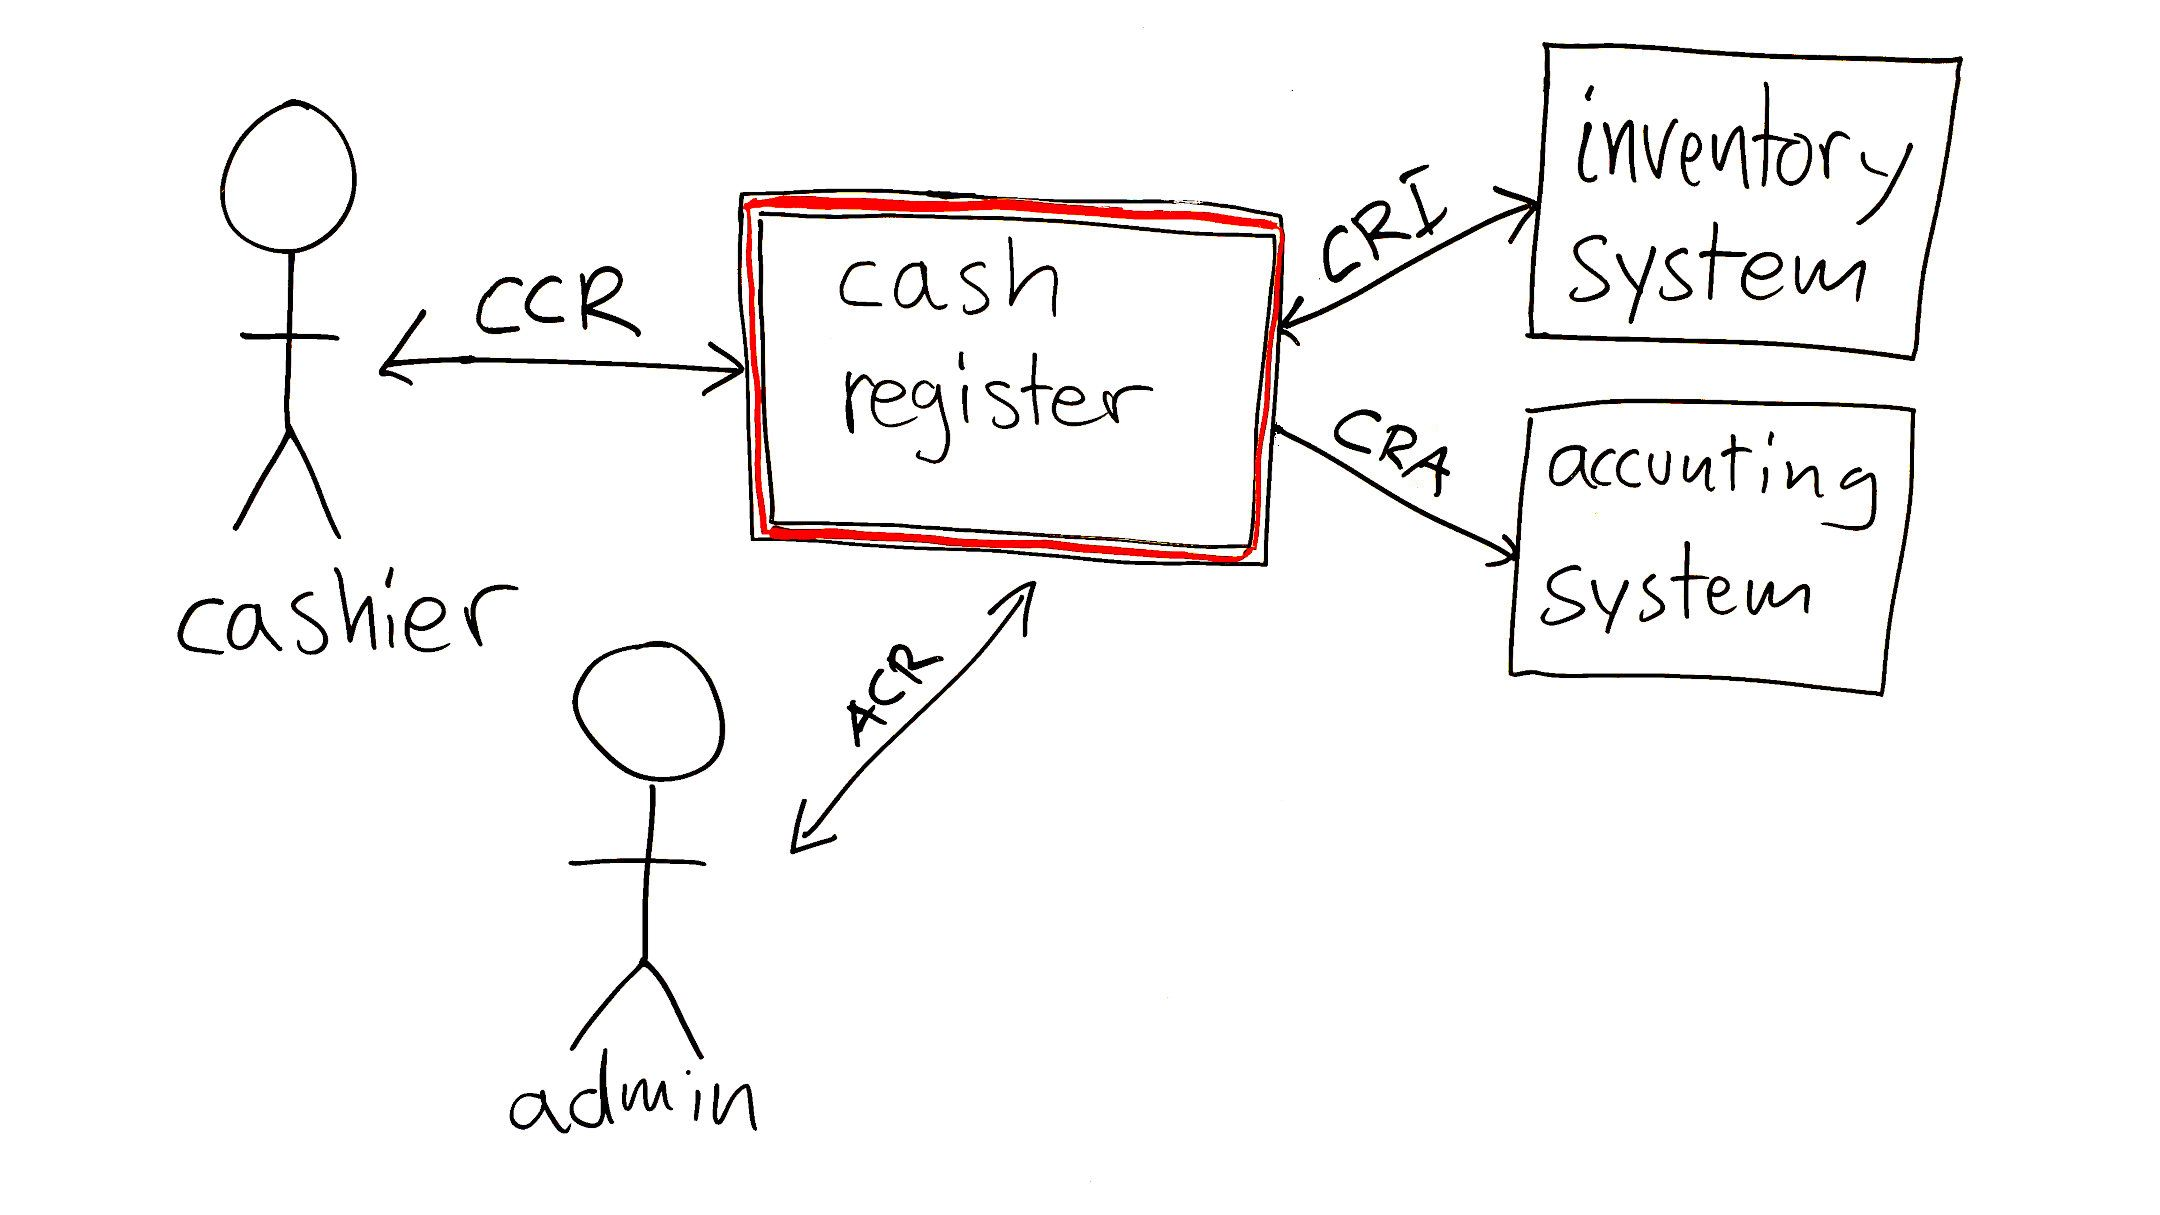
\includegraphics[width=0.9\textwidth]{../img/context-diagram-example}
\end{minipage}%
\vspace{1em}
\texttt{*~Interface~CRA}:\\ 
  \texttt{~~*~Spec:~The system shall ...~data entities ...}
\end{Slide}

\LectureOnly{\section{Elicitation}}
\begin{Slide}{What is requirements elicitation?}
\begin{itemize}
\item Engaging with stakeholders
\item Building domain knowledge
\item Discovering and inventing requirements
\item Exploring contextual usage
\item Starting-points: 
\begin{itemize}
\item Stakeholder Analysis
\item Context Diagram
\item Product Scoping

\end{itemize}
\end{itemize}
\end{Slide}
\begin{Slide}{Why is elicitation so hard?}
Elicitation challenges: Stakeholders often...
\begin{itemize}
\item cannot abstract 
\begin{itemize}
\item difficult to explain what they do and why
\item difficult to express what they (really) need
\item ask for specific solutions
\end{itemize}
\item lack imagination 
\begin{itemize}
\item of new ways of working
\item of consequences of new solutions
\end{itemize}
\item complicate the picture
\begin{itemize}
\item have conflicting demands
\item actively resist change
\item have luxury demands, ''gold plating''
\item have new demands once others are met

\end{itemize}
\end{itemize}
\end{Slide}
\begin{Slide}{Elicitation Methods}
%* Stakeholder analysis part of context
\begin{itemize}
\item Overview of elicitation methods: 
\begin{itemize}
\item Surveys
\item Interviews
\item Case-studies, examples:  demos, usability tests
\item Creativity methods, example: brainstorming, focus groups
    %* Brainstorming – generate ideas, creativity games
    %* Focus groups – gather a group of stakeholders
\item Operation Data Analysis: example: telemetry
    %* Usage statistics, telemetry
    %* User experiments, A/B-testing
    %* Feedback from marketing and support
    %* User and developer communities
    %* Mining social media
\item Business Intelligence: observing competitors 

\end{itemize}
\item Elicitation methods support specification, validation and selection, example: focus groups support selection, usability testing support validation

\end{itemize}
\end{Slide}
\begin{Slide}{Surveys}
\begin{itemize}
\item Good for asking many persons to get an overview of distribution of views
\item \TODO topics to consider
\begin{itemize}
\item Population definition and sampling
\item Response rate
\item Closed and open questions
\item Lickert Scale
\item statistics, correlation, etc.


\end{itemize}
\end{itemize}
\end{Slide}
\begin{Slide}{Interviews}
\begin{itemize}
\item Unstructured interviews: open questions, open topics
\item Structured interviews: closed questions, focused topics
\item Semi-structured: combine both


\end{itemize}
\end{Slide}
\begin{Slide}{Case Studies with Stakeholders}
\begin{itemize}
\item Demonstrations by stakeholders
\begin{itemize}
\item task enactment in a specific usage context
\end{itemize}
\item Observation of stakeholders 
\begin{itemize}
\item sometimes it is easier to show than tell
\end{itemize}
\item Prototyping (has its own chapter) 
\item Usability testing (has its own chapter)
\item Pilot product deployment
\begin{itemize}
\item limited but real usage of system in production
\item sometimes deployment is higher risk than development

\end{itemize}
\end{itemize}
\end{Slide}
\begin{Slide}{Operation Data Analysis}
Observe system in production before subsequent evolution
\begin{itemize}
\item Usage statistics, telemetry
\item Online user experiments, A/B-testing
\item Feedback from marketing
\item Feedback from support
\item Engage with user communities
\item Mining social media

\end{itemize}
\end{Slide}
\begin{Slide}{Creativity Methods}
Group activities that support innovation.
\begin{itemize}
\item Purposes: 
\begin{itemize}
\item trigger change and give competitive advantage
\item facilitate stakeholders in idea generation and assessment
\item get feedback on novelty and market opportunities
\end{itemize}
\item Example methods:
\begin{itemize}
\item Brainstorming: free-form idea generation without assessment
\item Focus-groups: structured brainstorming with assessment
\item Creativity Workshops: explore, combine, transform


\end{itemize}
\end{itemize}
\end{Slide}
\begin{Slide}{Creativity Workshops}
Workshops based on applied creativity theory including:
\begin{itemize}
\item Exploratory phase: opening up the space of ideas
\item Combinatorial phase: combining ideas to generate new ones
\item Transformational phase: 
\begin{itemize}
\item change problem space so something that is impossible now becomes possible
\end{itemize}
\item Analogical reasoning: 
\begin{itemize}
\item transfer knowledge from analogical domain
\end{itemize}
\item Storyboarding: 
\begin{itemize}
\item integrate ideas related to selected use cases


\end{itemize}
\end{itemize}
\end{Slide}
\LectureOnly{\section{Prioritization}}
\begin{Slide}{Requirements Selection}
\begin{itemize}
\item Requirements Selection provide input to downstream activities, answering the question: 
\begin{itemize}
\item What features are currently in and out of scope?
\end{itemize}
\item Requirements selection includes:
\begin{itemize}
\item \textbf{Prioritization} 
\begin{itemize}
\item ranking of requirements based on aspects such as benefit, cost, risk
\end{itemize}
\item \textbf{Product Scoping} (own chapter)
\begin{itemize}
\item Defining the scope and theme of each release
\item Release Planning: deciding the feature set included in each release, while taking into account resource constraints and priorities


\end{itemize}
\end{itemize}
\end{itemize}
\end{Slide}
\begin{Slide}{Why Prioritize?}
\begin{itemize}
\item To focus on the most important issues
\item To find high and low priority requirements
\item To implement requirements in a good order
\item To save time and money

\end{itemize}
\end{Slide}
\begin{Slide}{Prioritization steps}
\begin{itemize}
\item Select prioritization aspects (e.g. benefit, cost, risk)
\item Select prioritization objects (e.g., features)
\begin{itemize}
\item Try to define features at a high-enough level that can be selected or de-selected independently (if possible)
\end{itemize}
\item Structure and groups objects
\item Do the actual prioritization
\begin{itemize}
\item Decide priorities for each aspect, for each object
\end{itemize}
\item Visualize, discuss, iterate...

\end{itemize}
\end{Slide}
\begin{Slide}{Why is prioritization hard?}
Prioritization challenges:
\begin{itemize}
\item Finding a good abstraction level
\item Combinatorial explosion
\item Inter-dependencies
\item Not easy to predict the future
\item Power and politics

\end{itemize}
\end{Slide}
\begin{Slide}{Prioritization Aspects}
Examples of prioritzation aspects:
\begin{itemize}
\item Importance (e.g. financial benefit, urgency, strategic value, market share...)
\item Penalty (e.g. bad-will if requirement not included)
\item Cost (e.g., staff effort)
\item Time (e.g., lead time)
\item Risk (e.g., technical risk, business risk)
\item Volatility (e.g. scope instability, probability of change)
\item Other things to consider: 
\begin{itemize}
\item competitors, brand fitness, competence, release theme
\end{itemize}
\item Combine and optimize aspects, e.g.:
\begin{itemize}
\item cost vs. benefit, cost vs. risk, importance vs. volatility
\item maximizing benefit while minimizing cost

\end{itemize}
\end{itemize}
\end{Slide}
\begin{Slide}{When to prioritize?}
\begin{itemize}
\item Before spending large RE effort on a specific feature
\item At decision points, e.g.,
\begin{itemize}
\item Start of feature design
\item Start of feature implementation
\item Release Planning
\end{itemize}
\item When big changes occur
\item Regularly with \textit{lagom} intervals


\end{itemize}
\end{Slide}
\begin{Slide}{Who should prioritize?}
Find the right competence for the right aspect
\begin{itemize}
\item \textbf{Developers} know about e.g., 
\begin{itemize}
\item development effort and engineering risk
\end{itemize}
\item \textbf{Support} organization knows about e.g., 
\begin{itemize}
\item customer value if included and cost penalty if excluded
\end{itemize}
\item \textbf{Marketing} organization knows e.g., 
\begin{itemize}
\item competitors' products, market opportunities, cost of sales
\end{itemize}
\item etc...

\end{itemize}
\end{Slide}
\begin{Slide}{Prioritization Scales}
\begin{itemize}
\item For each aspect you need to decide on a metric
\item A metric is expressed/estimated using a value on a \textbf{scale}
\item Different types of scales with different power:
\begin{itemize}
\item categorical scale $\{A, B, C\}$ 
\begin{itemize}
\item example: \{must, ambiguous, volatile\}
\end{itemize}
\item ordinal scale $A > B$
\begin{itemize}
\item examples: higher value, more expensive
\end{itemize}
\item ratio scale $A = k \cdot B$
\begin{itemize}
\item examples: amount of money, hours, percentage

\end{itemize}
\end{itemize}
\end{itemize}
\end{Slide}
\begin{Slide}{Prioritization Methods}
Different methods, can be combined
\begin{itemize}
\item Grouping, categorical scale  
\begin{itemize}
\item example: use post-it notes on a white-board to group interdependent features
\end{itemize}
\item Top-$N$, e.g. $N = 5$, categorical combined with ordinal
\begin{itemize}
\item example: select 5 most beneficial features from the viewpoint of a specific stakeholder
\end{itemize}
\item Grading on an ordinal scale
\begin{itemize}
\item examples: grading 1...5, high--medium--low
\end{itemize}
\item Ordering by pair-wise comparison (sorting, ordinal scale)
\begin{itemize}
\item use insertion sort to arrange in order of highest to lowest risk
\end{itemize}
\item 100-dollar-test, ratio-scale
\begin{itemize}
\item distribute fictitious money to reflect prioritization aspect

\end{itemize}
\end{itemize}
\end{Slide}
\begin{Slide}{Prioritization Methods Combined}
Example of how prioritization techniques can be combined:
\begin{itemize}
\item Start with a high-level grouping of features that are highly interdependent to reduce the number of prioritization objects
\item Sort all features of small groups in benefit order
\item Use Top-5 for groups with large number of features
\item For selected groups that are most important for the coming release:
  do a ratio-scale prioritization with the 100-dollar-test

\end{itemize}
\end{Slide}
\begin{Slide}{Prioritization as Constraint Solving}

\begin{itemize}
\item \TODO{Part of lab}
\item \TODO{discuss circular inconsistency in pair-wise comparison}







\end{itemize}
\end{Slide}
\end{document}